% ------------------------------------------------------------------------
% ------------------------------------------------------------------------
% Modelo UFSC para Trabalhos Academicos (tese de doutorado, dissertação de
% mestrado) utilizando a classe abntex2
%
% Autor: Alisson Lopes Furlani
% 	Modificações:
%	- 27/08/2019: Alisson L. Furlani, add pacote 'glossaries' para listas
% - 30/10/2019: Alisson L. Furlani, adjusted some spacing errors and changed math fonts
% - 17/01/2019: Alisson L. Furlani, updated certification page
% - 03/03/2020: Luiz F. P. Droubi, change file to be used as a template with R.
% ------------------------------------------------------------------------
% ------------------------------------------------------------------------

\documentclass[
	% -- opções da classe memoir --
	12pt,				% tamanho da fonte
	%openright,			% capítulos começam em pág ímpar (insere página vazia caso preciso)
	oneside,			% para impressão no anverso. Oposto a twoside
	a4paper,			% tamanho do papel.
	% -- opções da classe abntex2 --
	chapter=TITLE,		% títulos de capítulos convertidos em letras maiúsculas
	section=TITLE,		% títulos de seções convertidos em letras maiúsculas
	%subsection=TITLE,	% títulos de subseções convertidos em letras maiúsculas
	%subsubsection=TITLE,% títulos de subsubseções convertidos em letras maiúsculas
	% -- opções do pacote babel --
	english,			% idioma adicional para hifenização
	%french,				% idioma adicional para hifenização
	%spanish,			% idioma adicional para hifenização
	brazil				% o último idioma é o principal do documento
	]{abntex2}

\usepackage{setup/ufrnthesisA4-alf}

\addbibresource{bib/thesis.bib}
\addbibresource{bib/discussion.bib}
\addbibresource{bib/pkgs.bib}

\usepackage[table]{xcolor}
\let\newfloat\undefined
\usepackage{floatrow}
\floatsetup[table]{capposition=top}
\floatsetup[figure]{capposition=top}

\newcommand{\pkg}[1]{{\normalfont\fontseries{b}\selectfont #1}}
\let\proglang=\textsf
\let\code=\texttt


\newcommand{\bcenter}{\begin{center}}
\newcommand{\ecenter}{\end{center}}

\newcommand{\bapendices}{\begin{apendicesenv}}
\newcommand{\eapendices}{\end{apendicesenv}}

\newcommand{\banexos}{\begin{anexosenv}}
\newcommand{\eanexos}{\end{anexosenv}}

% ---
% Filtering and Mapping Bibliographies
% ---
\DeclareSourcemap{
	\maps[datatype=bibtex]{
		% remove fields that are always useless
		\map{
			\step[fieldset=abstract, null]
			\step[fieldset=pagetotal, null]
		}
		% remove URLs for types that are primarily printed
%		\map{
%			\pernottype{software}
%			\pernottype{online}
%			\pernottype{report}
%			\pernottype{techreport}
%			\pernottype{standard}
%			\pernottype{manual}
%			\pernottype{misc}
%			\step[fieldset=url, null]
%			\step[fieldset=urldate, null]
%		}
		\map{
			\pertype{inproceedings}
			% remove mostly redundant conference information
			\step[fieldset=venue, null]
			\step[fieldset=eventdate, null]
			\step[fieldset=eventtitle, null]
			% do not show ISBN for proceedings
			\step[fieldset=isbn, null]
			% Citavi bug
			\step[fieldset=volume, null]
		}
	}
}
% ---

% ---
% Informações de dados para CAPA e FOLHA DE ROSTO
% ---
% FIXME Substituir 'Nome completo do autor' pelo seu nome.
\autor{JOÃO VITOR FERREIRA CAVALCANTE}
% FIXME Substituir 'Título do trabalho' pelo título da trabalho.
\titulo{O Ecossistema Computacional da Metagenômica}
% FIXME Substituir 'Subtítulo (se houver)' pelo subtítulo da trabalho.
% Caso não tenha substítulo, comente a linha a seguir.
  \subtitulo{Fluxos de Trabalho, Reprodutibilidade e Replicabilidade}
% FIXME Substituir 'XXXXXX' pelo nome do seu
% orientador.
\orientador{Rodrigo Juliani Siqueira Dalmolin}
% FIXME Se for orientado por uma mulher, comente a linha acima e descomente a linha a seguir.
% \orientador[Orientadora]{Nome da orientadora, Dra.}
% FIXME Substituir 'XXXXXX' pelo nome do seu
% coorientador. Caso não tenha coorientador, comente a linha a seguir.
% FIXME Se for coorientado por uma mulher, comente a linha acima e descomente a linha a seguir.
% \coorientador[Coorientadora]{XXXXXX, Dra.}
% FIXME Substituir '[ano]' pelo ano (ano) em que seu trabalho foi defendido.
\ano{2025}
% FIXME Substituir '[dia] de [mês] de [ano]' pela data em que ocorreu sua defesa.
\data{31 de Setembro de 2025}
% FIXME Substituir 'Local' pela cidade em que ocorreu sua defesa.
\local{NATAL - RN}
\instituicaosigla{UFRN}
\instituicao{Universidade Federal do Rio Grande do Norte}
% FIXME Substituir 'Dissertação/Tese' pelo tipo de trabalho (Tese, Dissertação).
\tipotrabalho{Defesa de Mestrado}
% FIXME Substituir '[mestre/doutor] em XXXXXX' pela grau adequado.
\formacao{Mestre em Bioinformática}
% FIXME Substituir '[mestrado/doutorado]' pelo nivel adequado.
\nivel{mestrado}
% FIXME Substituir 'Programa de Pós-Graduação em XXXXXX' pela curso adequado.
\programa{Programa de Pós-Graduação em Bioinformática}
% FIXME Substituir 'Campus XXXXXX ou Centro de XXXXXX' pelo campus ou centro adequado.
\centro{Instituto Metrópole Digital}
\preambulo
{%
\imprimirtipotrabalho~apresentada~ao~\imprimirprograma~da~\imprimirinstituicao.
}
% ---

% ---
% Configurações de aparência do PDF final
% ---
% alterando o aspecto da cor azul
\definecolor{blue}{RGB}{41,5,195}
% informações do PDF
\makeatletter
\hypersetup{
     	%pagebackref=true,
		pdftitle={\@title},
		pdfauthor={\@author},
    	pdfsubject={\imprimirpreambulo},
	    pdfcreator={LaTeX with abnTeX2},
		pdfkeywords={ufsc, latex, abntex2},
		colorlinks=true,       		% false: boxed links; true: colored links
    	linkcolor=black,%blue,          	% color of internal links
    	citecolor=black,%blue,        		% color of links to bibliography
    	filecolor=black,%magenta,      		% color of file links
		urlcolor=black,%blue,
		bookmarksdepth=4
}
\makeatother
% ---

% ---
% compila a lista de abreviaturas e siglas e a lista de símbolos
% ---

% Declaração das siglas
\siglalista{MS}{metagenômica \textit{shotgun}}
\siglalista{16S}{sequenciamento da subunidade ribossomal 16S de genomas bacterianos}
\siglalista{TDM}{transtorno depressivo maior}
\siglalista{DNA}{Ácido Desoxirribonucléico}
\siglalista{OTU}{unidades taxonômicas operacionais - do inglês \textit{operational taxonomic units}}
\siglalista{ASV}{variantes de sequência amplicon - do inglês \textit{amplicon sequence variant}}


% Declaração dos simbolos
\simbololista{C}{\ensuremath{C}}{Circunferência de um círculo}
\simbololista{pi}{\ensuremath{\pi}}{Número pi}
\simbololista{r}{\ensuremath{r}}{Raio de um círculo}
\simbololista{A}{\ensuremath{A}}{Área de um círculo}


% compila a lista de abreviaturas e siglas e a lista de símbolos
\makenoidxglossaries

% ---

% ---
% compila o indice
% ---
\makeindex
% ---

% ----
% Início do documento
% ----
\begin{document}

% Seleciona o idioma do documento (conforme pacotes do babel)
%\selectlanguage{english}
\selectlanguage{brazil}

% Retira espaço extra obsoleto entre as frases.
\frenchspacing

% Espaçamento 1.5 entre linhas
\OnehalfSpacing

% Corrige justificação
%\sloppy

% ----------------------------------------------------------
% ELEMENTOS PRÉ-TEXTUAIS
% ----------------------------------------------------------
% \pretextual %a macro \pretextual é acionado automaticamente no início de \begin{document}
% ---
% Capa, folha de rosto, ficha bibliografica, errata, folha de apróvação
% Dedicatória, agradecimentos, epígrafe, resumos, listas
% ---
% ---
% Capa
% ---
\imprimircapa
% ---

% ---
% Folha de rosto
% (o * indica que haverá a ficha bibliográfica)
% ---
\imprimirfolhaderosto*
% ---

% ---
% Inserir a ficha bibliografica
% ---
% http://ficha.bu.ufsc.br/
% \begin{fichacatalografica}
% 	\includepdf{Ficha_Catalografica.pdf}
% \end{fichacatalografica}
% ---

% ---
% Inserir folha de aprovação
% ---
\begin{folhadeaprovacao}
	\OnehalfSpacing
	% \centering
	\begin{center}
	\imprimirautor\\%
	\vspace*{10pt}
	\textbf{\imprimirtitulo}%
	\ifnotempty{\imprimirsubtitulo}{:~\imprimirsubtitulo}\\%
	%		\vspace*{31.5pt}%3\baselineskip
	\vspace*{\baselineskip}
	\end{center}
	%\begin{minipage}{\textwidth}
	\imprimirtipotrabalho~apresentada~ao~\imprimirprograma~da~\imprimirinstituicao\\
	%\end{minipage}%
	\bigskip\newline
	\textbf{Área de Concentração}:~Bioinformática\newline%
	\textbf{Linha de Pesquisa}:~Biologia de Sistemas\newline%
	\imprimirorientadorRotulo:~\imprimirorientador\newline%
	\begin{flushright}
	Natal, \imprimirdata.
	\end{flushright}
	\vspace*{\baselineskip}
  %   % Prof. Renan Cipriano Moioli, Dr.\\
  % Universidade Federal do Rio Grande do Norte - UFRN\\
  % \vspace*{\baselineskip}
  %   % Prof. Daniel Carlos Ferreira Lanza, Dr.\\
  % Universidade Federal do Rio Grande do Norte - UFRN\\
  % \vspace*{\baselineskip}
  %   % Prof. Marcel da Câmara Ribeiro-Dantas, Dr.\\
  % Universidade Potiguar - UNP\\
  % \vspace*{\baselineskip}
  % 
	\vspace*{2\baselineskip}
	% \begin{minipage}{\textwidth}
	% 	Certificamos que esta é a \textbf{versão original e final} do trabalho de conclusão que foi julgado adequado para obtenção do título de \imprimirformacao.\\
	% \end{minipage}
	%    \vspace{-0.7cm}
	\centering{\textbf{BANCA EXAMINADORA}}
	\assinatura{\OnehalfSpacing Prof. Dr. \imprimirorientador \\ \footnotesize{\imprimirinstituicao \\ (Presidente)}}
    \assinatura{Prof. Dr. Renan Cipriano Moioli \\ \footnotesize{Universidade Federal do Rio Grande do Norte \\ (Examinador Interno do Programa)}}
    \assinatura{Prof. Dr. Daniel Carlos Ferreira Lanza \\ \footnotesize{Universidade Federal do Rio Grande do Norte \\ (Examinador Interno do Programa)}}
    \assinatura{Prof. Dr. Marcel da Câmara Ribeiro-Dantas \\ \footnotesize{Universidade Potiguar \\ (Examinador Externo à Instituição)}}
  	%	\ifnotempty{\imprimircoorientador}{
	%	\assinatura{\imprimircoorientador \\ \imprimircoorientadorRotulo \\
	%		\imprimirinstituicao~--~\imprimirinstituicaosigla}
	%	}
	% \newpage
	\vspace*{\fill}
	\centering
\end{folhadeaprovacao}
% ---

% ---
% Dedicatória
% ---
\begin{dedicatoria}
	\vspace*{\fill}
	\noindent
	\begin{adjustwidth*}{}{5.5cm}
		\raggedleft
		Non ut sit repellendus ea sunt dolor.
	\end{adjustwidth*}
\end{dedicatoria}
% ---

% ---
% Agradecimentos
% ---
\begin{agradecimentos}
	Nihil ipsum velit cupiditate. Facilis inventore eveniet illo et.\\
Fugit unde cumque necessitatibus repudiandae non.\\
Voluptatem hic a numquam enim aperiam voluptatem.
\end{agradecimentos}
% ---

% ---
% Epígrafe
% ---
\begin{epigrafe}
	\vspace*{\fill}
	\begin{flushright}
		\textit{``Eppur si muove!''\\
(Galileu Galilei, 1633)}
	\end{flushright}
\end{epigrafe}
% ---

% ---
% RESUMOS
% ---

% resumo em português
\setlength{\absparsep}{18pt} % ajusta o espaçamento dos parágrafos do resumo
\begin{resumo}
	\SingleSpacing
  No resumo são ressaltados o objetivo da pesquisa, o método utilizado, as discussões e os resultados com destaque apenas para os pontos principais. O resumo deve ser significativo, composto de uma sequência de frases concisas, afirmativas, e não de uma enumeração de tópicos. Não deve conter citações. Deve usar o verbo na voz ativa e na terceira pessoa do singular. O texto do resumo deve ser digitado, em um único bloco, sem espaço de parágrafo. O espaçamento entre linhas é simples e o tamanho da fonte é 12. Abaixo do resumo, informar as palavras-chave (palavras ou expressões significativas retiradas do texto) ou, termos retirados de thesaurus da área. Deve conter de 150 a 500 palavras. O resumo é elaborado de acordo com a NBR 6028.

  \textbf{Palavras-chave}:
    Palavra-chave 1.
    Palavra-chave 2.
  \end{resumo}
% resumo em inglês
\begin{resumo}[Abstract]
	\SingleSpacing
	\begin{otherlanguage*}{english}
		Resumo traduzido para outros idiomas, neste caso, inglês. Segue o formato do resumo feito na língua vernácula. As palavras-chave traduzidas, versão em língua estrangeira, são colocadas abaixo do texto precedidas pela expressão ``Keywords'', separadas por ponto.

		\textbf{Keywords}:
	      Keyword 1.
        Keyword 2.
    	\end{otherlanguage*}
\end{resumo}
%% resumo em francês
%\begin{resumo}[Résumé]
% \begin{otherlanguage*}{french}
%    Il s'agit d'un résumé en français.
%
%   \textbf{Mots-clés}: latex. abntex. publication de textes.
% \end{otherlanguage*}
%\end{resumo}
%
%% resumo em espanhol
%\begin{resumo}[Resumen]
% \begin{otherlanguage*}{spanish}
%   Este es el resumen en español.
%
%   \textbf{Palabras clave}: latex. abntex. publicación de textos.
% \end{otherlanguage*}
%\end{resumo}
%% ---

{%hidelinks
	\hypersetup{hidelinks}
	% ---
	% inserir lista de ilustrações
	% ---
	\pdfbookmark[0]{\listfigurename}{lof}
	\listoffigures*
	\cleardoublepage
	% ---

	% ---
	% inserir lista de quadros
	% ---
	% \pdfbookmark[0]{\listofquadrosname}{loq}
	% \listofquadros*
	% \cleardoublepage
	% ---

	% ---
	% inserir lista de tabelas
	% ---
	\pdfbookmark[0]{\listtablename}{lot}
	\listoftables*
	\cleardoublepage
	% ---

	% ---
	% inserir lista de abreviaturas e siglas (devem ser declarados no preambulo)
	% ---
	\imprimirlistadesiglas
	% ---

	% ---
	% inserir lista de símbolos (devem ser declarados no preambulo)
	% ---
	% \imprimirlistadesimbolos
	% ---

	% ---
	% inserir o sumario
	% ---
	\pdfbookmark[0]{\contentsname}{toc}
	\tableofcontents*
	\cleardoublepage

}%hidelinks
% ---

% ---

% ----------------------------------------------------------
% ELEMENTOS TEXTUAIS
% ----------------------------------------------------------
\textual

\chapter{Introdução}\label{intro}

\section{Visão Geral - Metagenômica}\label{visuxe3o-geral---metagenuxf4mica}

A história da vida microscópica, ou microbiana, no planeta Terra supera a história da vida macroscópica por milhares de anos \autocite{magnabosco2024}. A metagenômica surge como uma abordagem que possibilita descobertas acerca da vida microbiana através do sequenciamento genético. Avanços no que viria eventualmente a se tornar a metagenômica surgem ainda nos anos 90, com o primeiro sequenciamento de genoma completo de um organismo de vida livre, a bactéria \emph{Haemophilus influenza} \autocite{wooley2010}. Esse ponto na história científica marca o primeiro uso bem sucedido do que vem a ser chamado de \emph{whole-genome shotgun}, ou sequenciamento de genoma completo, no qual a amostra possui seu conteúdo genético fragmentado em \emph{reads}, ou leituras, que são então sequenciadas. Essa técnica viria a ser refinada e aplicada para amostras ambientais, seja este ambiente uma amostra de solo florestal ou uma biópsia intestinal. Nessa nova técnica se buscou sequenciar o conteúdo genético que compreenda os diferentes microorganismos presentes em tais amostras, originando assim o que será aqui descrito como \gls{MS}.

No entanto, o estudo de comunidades microbianas se populariza de fato com uma técnica que não busca capturar o conteúdo genético total de uma amostra, mas apenas uma subregião de seu \gls{DNA} ribossomal que possua ao mesmo tempo regiões conservadas, capaz de serem passíveis de anelamento por \emph{primers}, e regiões hipervariáveis, capazes de distinguir um microorganismo de outro. Em bactérias o ribotipo selecionado foi o \gls{DNA} que codifica a subunidade 16S, que é amplificada e então sequenciada. O \gls{16S}, também denominado metataxonômica \autocite{marchesi2015}, possibilitou uma maneira simples, e pouco computacionalmente intensiva quando comparada à \gls{MS} \autocite{tremblay2022}, para realizar identificação de táxons bacterianos em uma amostra ambiental. Ademais, técnicas computacionais posteriores ultimamente facilitariam a conexão de informação funcional às abundâncias taxonômicas obtidas através desta técnica.

Dessa maneira, possuímos atualmente, duas possíveis abordagens para se estudar comunidades microbianas, a \gls{MS} e o \gls{16S}. Essas abordagens, por se basearem de aspectos distintos do microbioma, tipicamente são utilizadas de forma separada - e não integrativa - por estudos. Apesar disso, a integração de dados provenientes das duas abordagens pode auxiliar a remover vieses experimentais específicos de cada técnica, e, dessa maneira, conferir maior confiabilidade aos resultados \autocite{yue2023}.

\section{O Ecossistema computacional em Metagenômica}\label{o-ecossistema-computacional-em-metagenuxf4mica}

As metodologias de processamento de dados \gls{16S} em grande parte já estão estabelecidas, dada a idade mais avançada da abordagem. Nesse sentido, vemos que o cerne das abordagens trata de atribuir identificadores únicos às sequências 16S obtidas, caracterizando assim táxons distintos. Esses identificadores podem ser atribuídos através de métodos de agrupamento, caracterizando as abordagens baseadas em \gls{OTU}, que agrupam sequências com pelo menos 97\% de identidade em grupos biológicos distintos, ou abordagens baseadas em \gls{ASV}, que, através de modelos estatísticos, tentam definir variações biológicas reais na sequência - contrastadas com variações devido a erros de sequenciamento, e dessa maneira obter uma resolução taxonômica maior comparada às baseadas em \gls{OTU} \autocite{chiarello2022}. Nesse contexto, observamos metodologias que buscam, a partir dos \gls{OTU} ou \gls{ASV} identificados, inferir abundâncias de vias metabólicas específicas, tirando proveito de bancos de dados de informação curada a respeito desses táxons que possua mapeamento das famílias gênicas de seu genoma a funções biológicas \autocite{douglas2020}.

Por outro lado, o campo do desenvolvimento de metodologias para dados de \gls{MS} ainda é bastante fértil, com novas técnicas computacionais desenvolvidas rotineiramente \autocite{liu2021}. De forma geral, podemos agrupar as metodologias em duas grandes categorias: Metodologias livres de montagem, isto é, aquelas que se utilizam apenas da informação contidas nas leituras para obter seus resultados, e metodologias baseadas em montagem, que primeiro realizam a montagem de leituras em sequências contíguas (ou \textit{contigs}), que fornecerá então a base para o processamento seguinte \autocite{breitwieser2019}. Apesar da capacidade que métodos baseados em montagem tem de descobrir novos organismos e montar genomas inéditos, métodos livres de montagem apresentam certas vantagens, sobretudo quando consideramos dados com baixa cobertura de sequência, o que pode resultar em montagens pouco precisas \autocite{ayling2020}.

No que se diz respeito a essas metodologias, vemos que as baseadas em montagem são amplas e cobrem os mais diversos aspectos do processamento de dados de \gls{MS}, com exemplos como nf-core/mag \autocite{krakau2022} e metaphor \autocite{salazar2023}. No entanto, quando observamos métodos livres de montagem, vemos um cenário mais escasso, sobretudo quando consideramos apenas fluxos de trabalho, ou \emph{pipelines}, orquestrados por linguagems de gerenciamento de metodologias científicas, como Nextflow \autocite{ditommaso2017} ou Snakemake \autocite{mölder2021}, e que adiram a boas práticas de desenvolvimento de \emph{software} científico, como isolamento de dependências, instalação fácil e documentação descritiva, com exemplos \autocite{mangul2019}. No contexto de métodos livres de montagem para dados \gls{MS}, vale ressaltar o fluxo de trabalho MEDUSA \autocite{morais2022}, que apresentou boa sensitividade e flexibilidade para análises de classificação taxonômica e anotação funcional.

Nesse sentido, há a necessidade de desenvolver uma metodologia para dados de \gls{MS} que siga boas práticas de desenvolvimento de software e que tenha como princípios norteadores a reprodutibilidade, documentação expansiva e interpretabilidade. Este último ponto que se torna especialmente relevante ao considerarmos a complexidade e a alta dimensionalidade desses dados.

\section{Desenvolvimento de Software em Bioinformática}\label{desenvolvimento-de-software-em-bioinformuxe1tica}
\begin{itemize}
\tightlist
\item
  Princípios
\item
  Pipelines
\item
  Conteinerização
\item
  Reprodutibilidade e replicabilidade
\end{itemize}
\chapter{Objetivos}\label{obj}

\section{Geral}\label{geral}

Obter uma visão geral do ecossistema computacional em metagenômica atual e como ele se associa
com princípios de desenvolvimento de software científico, desenvolvendo então uma metodologia
para dados de \gls{MS} que possibilite uma análisa metagenômica compreensiva, de forma reprodutível e flexível.

\section{Específicos}\label{especuxedficos}
\begin{itemize}
\tightlist
\item
  Avaliar o atual ferramentário computacional para dados de metagenômica e sua adesão a princípios de desenvolvimento de software sustentável.
\item
  Desenvolver uma metodologia robusta, flexível e acessível para análise de dados de \gls{MS}.
\end{itemize}
\chapter*{CAPÍTULO 1}\label{cap1}
\addcontentsline{toc}{chapter}{CAPÍTULO 1}
\begin{center}
\textbf{Artigo: Bridging the Gaps in Meta-Omic Analysis: Workflows and Reproducibility}
\bigskip\newline
Escrito por: João Vitor Ferreira Cavalcante, Iara Dantas de Souza, Diego Arthur de Azevedo Morais e Rodrigo Juliani Siqueira Dalmolin
\bigskip\newline
\textit{Artigo publicado no periódico OMICS: A Journal of Integrative Biology}

\end{center}
\begin{fichacatalografica}
    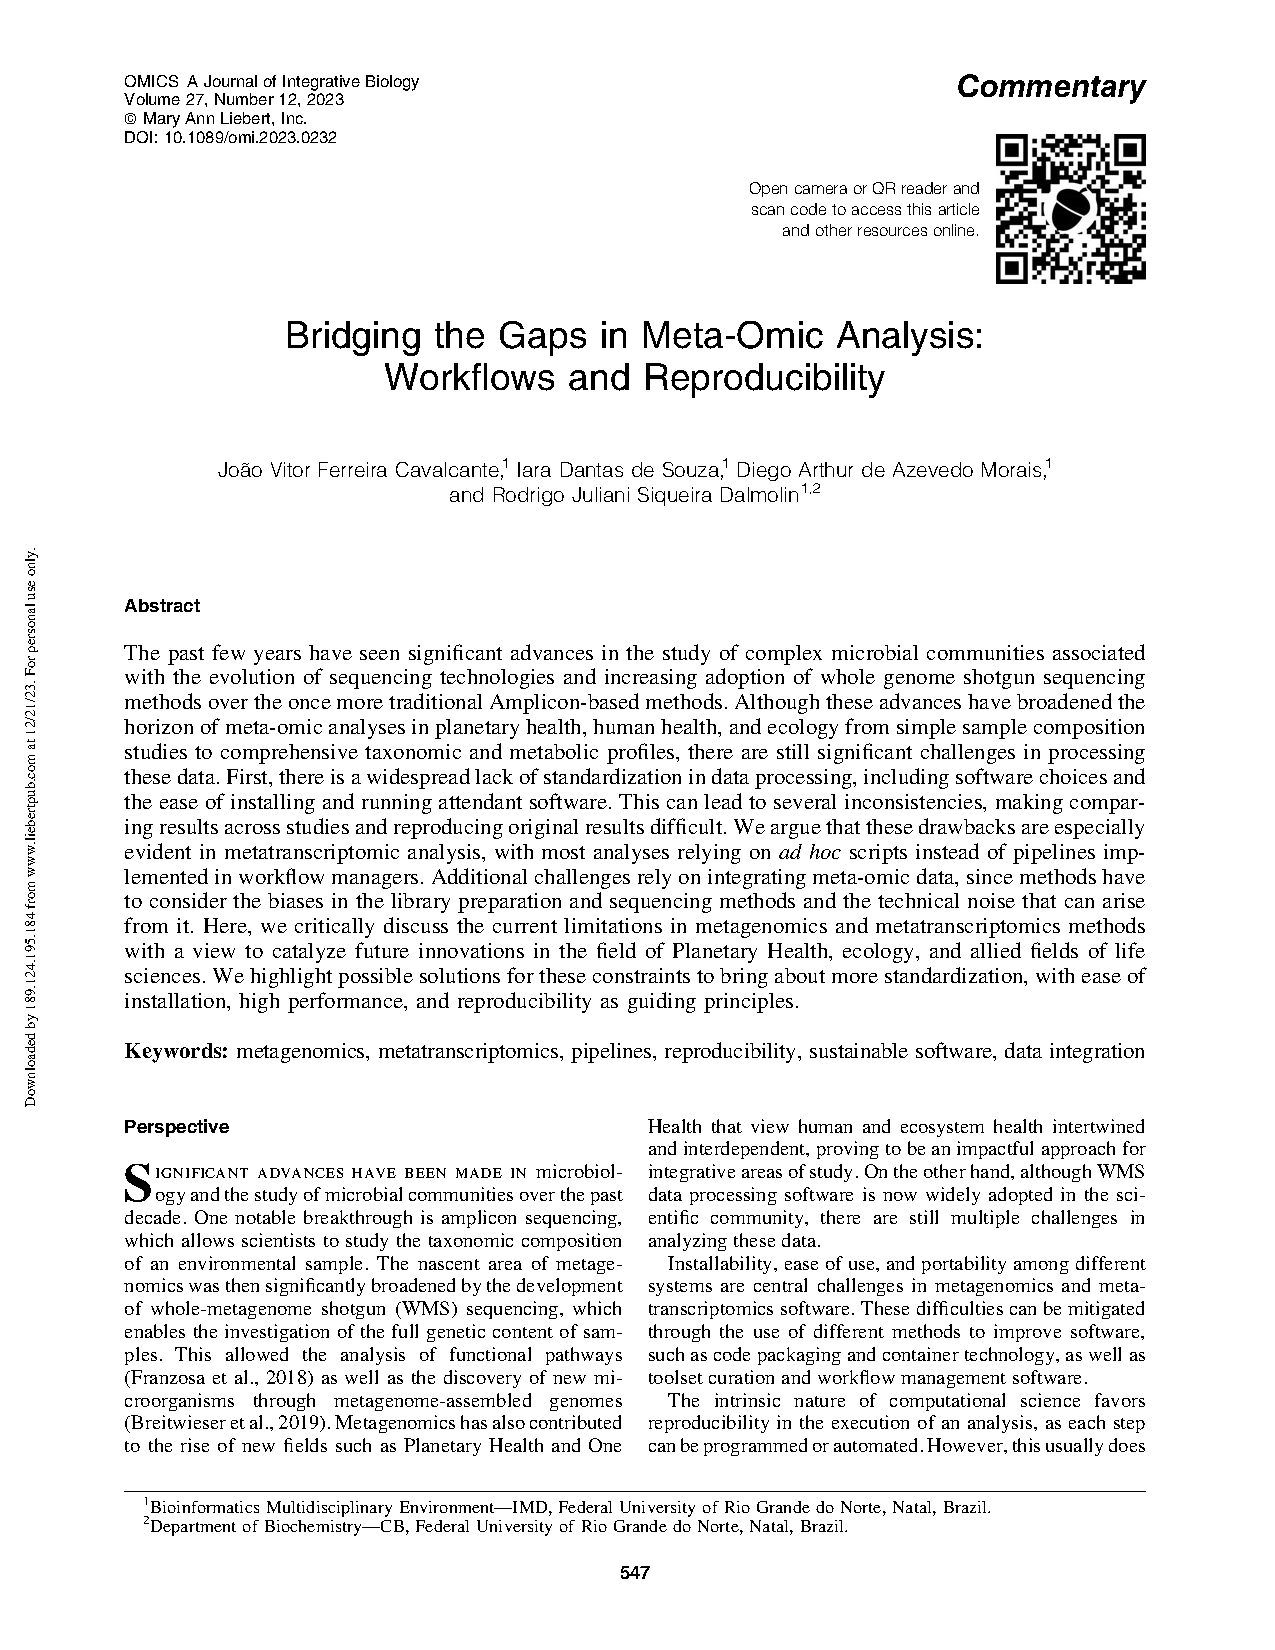
\includepdf[pages={1-}]{papers/paper1.pdf}
\end{fichacatalografica}
\chapter*{CAPÍTULO 2}\label{cap2}
\addcontentsline{toc}{chapter}{CAPÍTULO 2}
\begin{center}
\textbf{Artigo: EURYALE: A versatile Nextflow pipeline for taxonomic classification and functional annotation of metagenomics data}
\bigskip\newline
Escrito por: João Vitor Ferreira Cavalcante, Iara Dantas de Souza, Diego Arthur de Azevedo Morais e Rodrigo Juliani Siqueira Dalmolin
\bigskip\newline
\textit{Artigo submetido ao periódico IEEE Access}

\end{center}
\begin{fichacatalografica}
    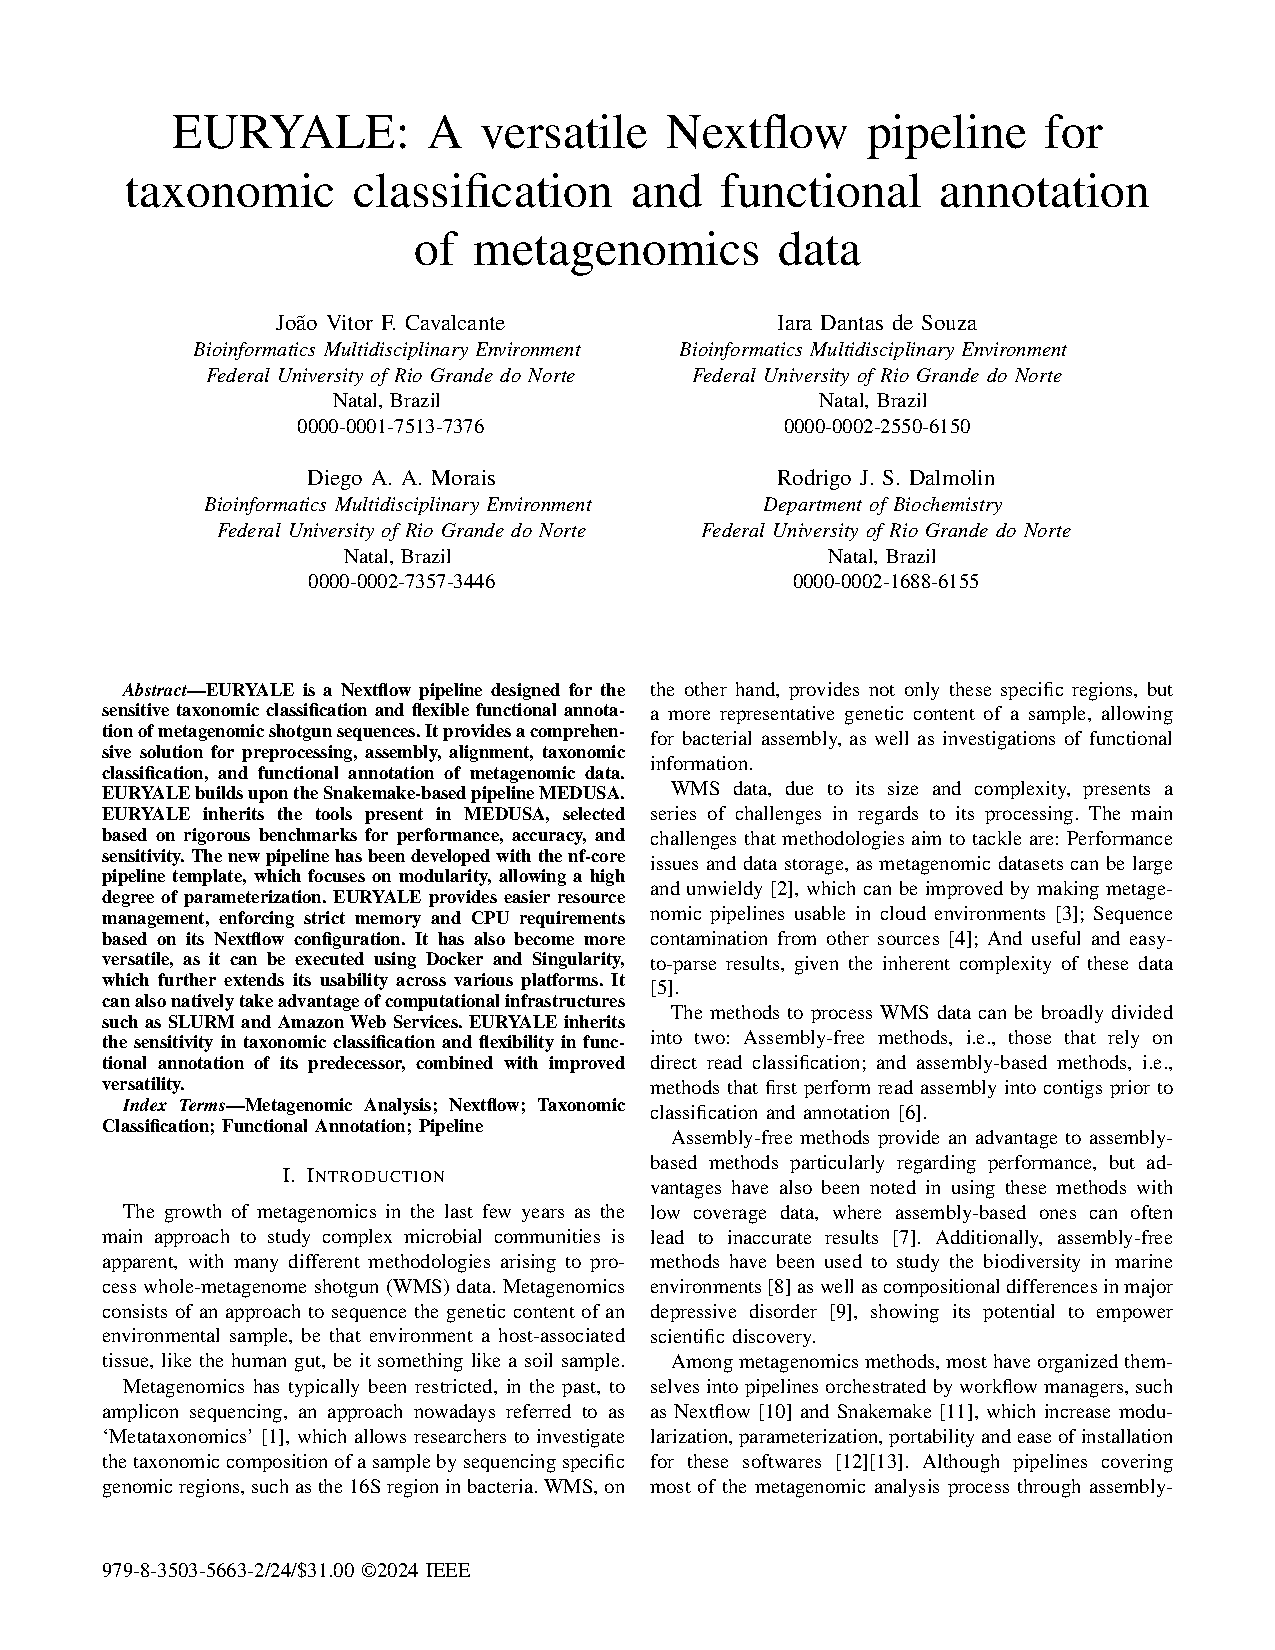
\includepdf[pages={1-}]{papers/paper2.pdf}
\end{fichacatalografica}
\chapter{Discussão}\label{disc}

Ao averiguarmos o estado da arte dos fluxos de trabalho computacional presentes na área da metagenômica, pudemos concluir que a adoção de tecnologias de conteinerização e orquestradores de execução ainda é um tanto limitada.
Essas limitações tornam-se mais evidentes sobretudo no contexto de metodologias de metagenômica livres de montagem.
Tais metodologias são mais escassas e menos computacionalmente intensas quando comparadas às abordagens baseadas em montagem.
Ainda assim, elas necessitam processamento adequado, de forma reprodutível, replicável e automatizável, especialmente por possibilitarem uma análise realizável em infraestruturas de menor porte e por possuírem melhor sensibilidade ao tratar dados com baixa cobertura \autocite{ayling2020}, ambos fatores comuns quando se tratando da produção e processamento de dados metagenômicos em ambientes com financiamento científico limitado, como no sul global.

No contexto de possíveis metodologias, decidimos então aplicar os princípios postos para a metodologia MEDUSA \autocite{morais2022}, que apresentou resultados superiores a fluxos de trabalho semelhantes, além de ter obtido suas ferramentas a partir de curadoria manual, com rigorosos processos de \emph{benchmarking}.
Portanto, tomando vantagem da curadoria precedente, decidimos então re-implementar o MEDUSA, utilizando-se agora do gerenciador de pipelines \emph{Nextflow} a de tecnologias de contêinerização: \emph{Docker} e \emph{Singularity. \textbf{A escolha do gerenciador\ldots{} Porquê conteinerização\ldots{}}}

\textbf{No entanto, acessibilidade ao usuário\ldots{} resultados de interpretabilidade complexa\ldots{} Detalhes sobre o MultiQC\ldots{} Microview e detalhes de sua implementação\ldots{} Figura ilustrativa do report microview\ldots{} Falar sobre como funciona isoladamente\ldots{}}

\textbf{Falar sobre nf-core\ldots{} alto grau de parametrização\ldots{} entry de download\ldots{}}

\chapter{Conclusão}\label{conclusuxe3o}

Ressaltar como avançamos nas metodologias de meta com orquestração e conteinerização,
priorizando princípios de software sustentável. Na mesma medida, nos baseamos em uma metodologia
sólida já existente, aprimorando nesses conceitos além de possibilitar melhor interpretabilidade
com a implementação de uma ferramenta adicional de reporting.
No entanto, faltar como metodologias de integração de dados metagenomica/metatranscriptomica ainda
são relativamente escassas, sobretudo considerando-se fluxos de trabalho automatizados e que sigam esses mesmos princípios.

\postextual

\begingroup

\printbibliography[title=REFERÊNCIAS]

\endgroup

\markboth{Referências}{REFERÊNCIAS}

% ----------------------------------------------------------
% Glossário
% ----------------------------------------------------------
%
% Consulte o manual da classe abntex2 para orientações sobre o glossário.
%
%\glossary

%---------------------------------------------------------------------
% INDICE REMISSIVO
%---------------------------------------------------------------------
%\phantompart
%\printindex
%---------------------------------------------------------------------

\end{document}
